\documentclass[10pt,a4paper]{article}
\usepackage[margin=1.6cm]{geometry}
\usepackage[latin1]{inputenc}
\usepackage{amsmath}
\usepackage{amsfonts}
\usepackage{amssymb}
\usepackage{multirow}
\usepackage{graphicx}
\usepackage{subcaption}
\usepackage{morefloats}

\setlength{\parskip}{5pt}
\setlength{\parindent}{0pt}

\author{Hector Dearman \and Paul Rowe-White \and Kritaphat Songsriin \and Simon Stuckemann}
\title{Machine Learning CBC: Neural Networks}
\begin{document}
\maketitle

\section{Implementation Details}

In order to create a multiple-output neural network and multiple single-output neural networks for clean and noisy datas, we wrote a script, {\tt make\_a\_net.m} (Figure~\ref{fig:optimise_6_output_net}), which load corresponding data and the pre-computed optimal parameters and perform a 10-fold cross validation on the entire exapmles. 

\subsection{Cross-Validation}

% Some more stuff here about implementation details

To validate the performance of our network we performed 10-fold cross validation. We performed 10 folds, each time splitting up our examples into a test and training set. In the first fold we then use 3-fold cross validation inside for each possible value of a parameter, each time splitting up our data into an actual training set and a validation set. As explained below we then use the training data to train a network and optimise the parameters against the validation set, choosing the parameter that performs best on average across all three folds. 

After fixing the parameters, from the first fold we then use the entire training data (everything except test data) to train a network and test its performance on the test set. In each fold, we record the confusion matrix so that we can calculate the average confusion matrix after all folds and then calculate the average recall rate, precision rate and $F_1$ measure as well as average error and classification rate. This approach is consistent with the approach we took in our first assignment.

\subsection{Classification}
Running the simulation of both types of networks results in a vector of six neural network outputs. These outputs are distributed around the values of 0 and 1, where those closer to 0 represent negative classifications and those around 1 positive classifications. In our implementation, to choose one of the emotions as our final classification, we select the emotion that returned the maximum raw output value of the network. Arguably, an approach that selects the output that is closest to the value 1 would be better -- however, we found that this slight modification does not change the results significantly.

\subsection{Pre-processing and Post-processing}



\section{Evaluation Process}

\subsection{Finding Optimal Parameters}
In order to find the optimal parameters for the neural network we ideally would have to perform an exhaustive search on all possible combinations. Since this is not feasible in the time we were given we made some simplifying assumptions that helped us decrease the evaluation time.

One of our most significant assumptions is independence of parameters. This is not a good assumption since clearly we will reach different conclusions when optimising the parameters in a different order, however, it is necessary to make the problem of optimising the parameters tractable.

We first set out each parameter we would have to optimise. To do this we listed all parameters and analysed the effect each parameter has on the result by fixing all other parameters, varying one parameter and observing the variance in the results. Having done this on a small subset of the data (1 fold) we concluded that the most influential parameters are \emph{training function}, \emph{number of nodes and layers}, \emph{goal}. % more here and do we want to write this? We didn't really do this...

In order to optimise the parameters we selected in the first step of the optimisation process, we implemented 3-fold cross validation inside the training set of the first fold, thus splitting the training set up into a new training set and a validation set and repeating the analysis three times, recording the average sum of the performance of one possible value for a parameter. After doing this for each of the possible parameter values we selected the value with the best performance measure.

Note that for most of the parameters it was possible to do a exhaustive (grid) search (after fixing a reasonable range and step size). However, for the topology of the network, the number of layers and the number of nodes within each layer, it still proved impractical to try every combination. To make optimising the topology possible in the time we had, we considered only topologies where every layer had the same number of nodes. In addition, we used a two layer search, first finding the best number of nodes to the nearest ten, then followed by a second search of the ten values on either side of the best result of the larger step\footnote{If the performance given by the number of nodes were modelled by a convex function this would result in the true optimum, but should also select a reasonably good value so long as the sensitivity of the parameter is relatively low.}.

Finally, as suggested in the specification of this coursework we only optimise the parameters in the first fold of the 10-fold cross validation. This means that we are fixing parameters that we obtained in another fold and we cannot actually be sure that the parameter values we found to be optimal are indeed optimal or whether they were influenced by fluctuations in the data set.

Ideally, this issue could be avoided by performing 10-fold cross validation in all folds. However, to be able to compare the optimal parameters in the end and pick the best, we would need to make sure that we always validate the optimal values against the same validation set. For this reason, we would fix a common validation that we could use in each fold. 10-fold cross validation is then performed on the rest of the data, always training the network on a training set, validating it against the fixed validation set and testing it on the test set. This process leads to having the choice between 10 different sets of parameters for a final network. To choose the best value for each parameter we can now choose the most common parameter in the set of optimal parameters.

The optimal values for the parameters we optimised can be found in table \

\begin{table}
\begin{tabular}{|r|c||c|c|c|c|c|c|}
\hline 
 & \textbf{6-output net} & \textbf{anger} & \textbf{disgust} & \textbf{fear} & \textbf{happiness} & \textbf{sadness} & \textbf{surprise} \\ 
\hline 
\textbf{layers} & $1$ & $3$ & $3$ & $2$ & $2$ & $3$ & $2$ \\ 
\hline 
\textbf{nodes} & $18$ & $26$ & $64$ & $28$ & $22$ & $81$ & $29$ \\ 
\hline 
\textbf{train function} & trainlm & trainlm & trainlm & trainlm & trainlm & trainlm & trainlm \\ 
\hline 
\textbf{epochs} & $835$ & $252$ &  & $399$ & $624$ &  & $706$ \\ 
\hline 
\textbf{goal} & $1e-4$ & $3e-4$ &  & $5e-4$ & $3e-4$ &  & $6e-4$ \\ 
\hline 
\textbf{max fail} & $4$ & $3$ &  & $4$ & $8$ &  & 9 \\ 
\hline 
\textbf{min grad} & $8.9e-7$ & $6.7e-7$ &  & $8e-8$ & $7.5e-7$ & & $4e-8$ \\ 
\hline 
\end{tabular} 
\caption{Optimal Parameter Values}
\label{tab:optimalValues}
\end{table}

\subsection{Performance measure}
For parameter optimisation, we Initially used the classification error as our performance measure. This worked when we were building the six-output network because the network produces multiple outputs and we can choose the classification with the highest certainty as our final classification (see above for explanation). However, when optimising the parameters for a one-output network this is difficult one would like to train and optimise each individual network without having to guess whether the particular output it gave would be enough to classify an example. 

To solve this issue we considered classifying outputs less than 0.5 negatively and outputs greater than or equal to 0.5 positively. However, this approach does not reflect the way we decide on a final classification. Furthermore, we would like to penalise or reward an output based on how right or how wrong it was: concretely, if an example were labelled 0 and we predicted 0.6, this is less bad (and our performance measure should give a better score) than if we predicted 1.0. 

To do this, we use the following logistic cost function:

\[
    Cost(p, y)= 
\begin{cases}
    -\log{p}& \text{if } y = 1\\
    -\log{(1 - p)}              & \text{if } y = 0
\end{cases}
\]

where $p$ is the prediction value of the neural network for an example and $y$ is its true label. Since the function accepts values between 0 and 1 and the raw output of the network is distributed around 0 or 1 but is not guaranteed to be in this range, we obtained the prediction value by applying the log sigmoid function to it, thus resulting in values between 0 and 1. 

Note, however, that in our case the split between positive and negative classifications for a given emotion is not 50:50. Since the examples are relatively balanced (the number of examples for each emotion is between 100 and 200), we can conclude that approximately $\frac{5}{6}$ of the examples will classify negatively and only $\frac{1}{6}$ will classify positively (see figure \ref{fig:examplesDistribution}).

\begin{figure}[!ht]
     \centering
     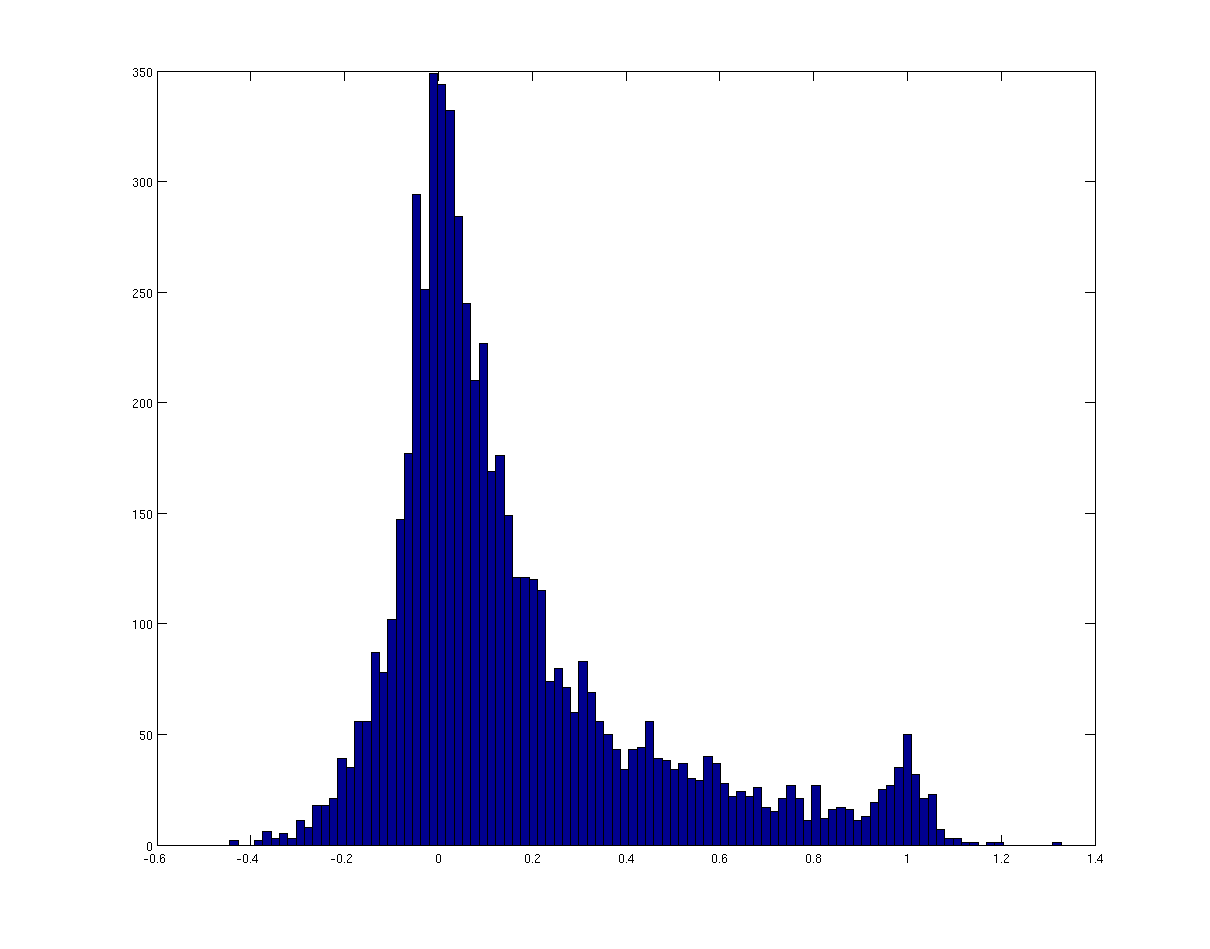
\includegraphics[scale=0.3]{../../images/clean_hist.png}
     \caption{Histogram of Neural Network Output}
     \label{fig:examplesDistribution}
\end{figure}

This distribution means that simply passing the raw value into the log sigmoid function will result in wrong cost values. For instance, if one of the networks' output were 0, this should result in a relatively low value after applying the log sigmoid function. However, since $logsig(0) = 0.5$ this is not the case and the network would be penalised unnecessarily. To avoid this, we shift the log sigmoid function to the right by 0.5 as this seems to be a reasonable cut-off point (see figure \ref{fig:examplesDistribution}).

To optimise the parameters, we take the sum of this cost function over every example in the validation set as our performance measure, meaning that during optimisation we tried to minimise this sum of costs. This new function gave very similar results to the previous measure on the six-output networks so we where confident it was not completely wrong.

\subsection{Avoiding Overfitting (2)}
The \emph{MATLAB} documentation suggests two ways to avoid overfitting: early stopping and regularisation. In our implementation we use the early stopping technique which uses a validation set to determine the right point at which to stop fitting the network to the training data. One of the parameters that this technique uses is \emph{max\_fail} which describes the maximum number of times the error rate in the validation set can increase before the training function stops. This parameter defaults to 6 and any changes we made did not seem to have a large impact on the end results.

Regularisation, on the other hand, involves modifying the performance function used by the training function by adding a term that consists of the mean of the sum of squares of the network weights and biases. This new performance function causes the network to have smaller weights and biases and forces the network response to be smoother and less likely to overfit.

\section{Results (3)}

\subsection{Average F1 Value Per Fold}
As can be seen in Figure~\ref{fig:avgF1} the average F1 value for the noisy data was lower than the average value F1 value for the clean data. Another difference is that on the clean data the set the single output networks trends above the six output network whereas on the noisy data this trend is reversed and the six output network trends higher than the set of single output networks. However there is not substantial difference between the two different types of network on either figure and there appears to be no more than $5-10\%$ difference in the F1 measure between the two.

\subsection{Comments on Results}

We can see that both types of networks consistantly classify happiness and sadness (emotions 4 and 6) with very high precision for both clean and noisy data. The other stand out result is that both types of network perform very poorly when trying to classify anger in noisy data.

any difference between the average classification performance of the two types, both clean and noisy data. Discuss advantages and disadvantages

Commented results on average confusion matrices for both types of network and both clean and noisy with 
	- avg. classification rate
	- recall rate, precision rate, and F1 per class

figures of the average performance per fold for both types and nosiy/clean; discussion

\begin{figure}[!ht]
	\centering
	\begin{subfigure}[b]{0.7\textwidth}
		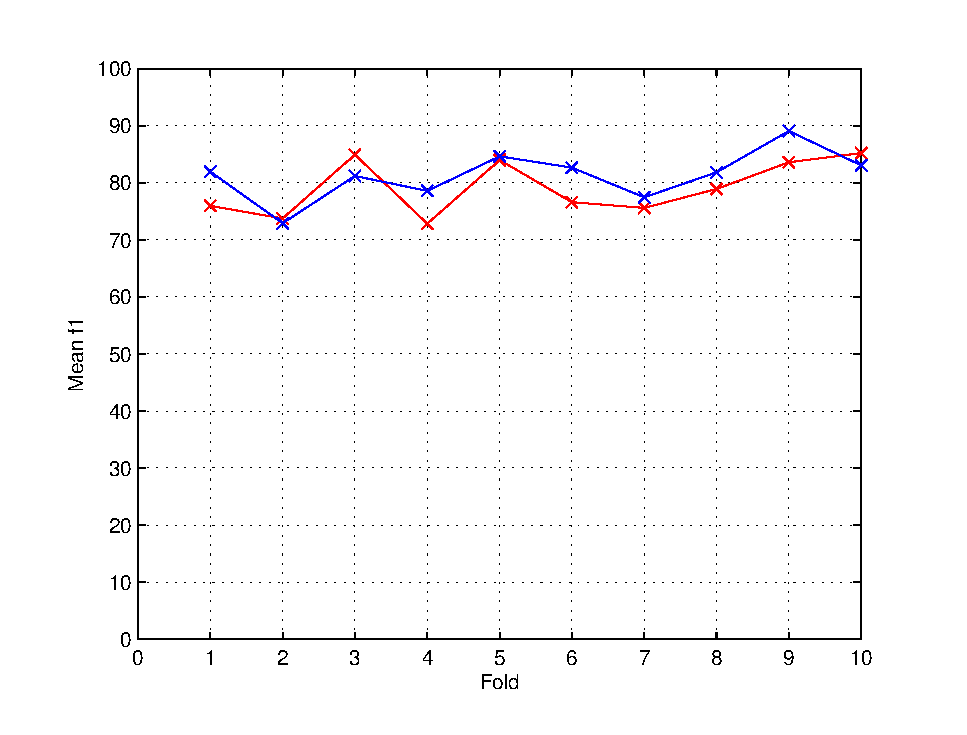
\includegraphics[width=\textwidth]{images/clean_fold_f1_plot.eps}
     	\caption{Average value of F1 measure for all 6 emotions against folds for clean data}
     	\label{fig:avgF1Clean}
    \end{subfigure}
	\begin{subfigure}[b]{0.7\textwidth}
		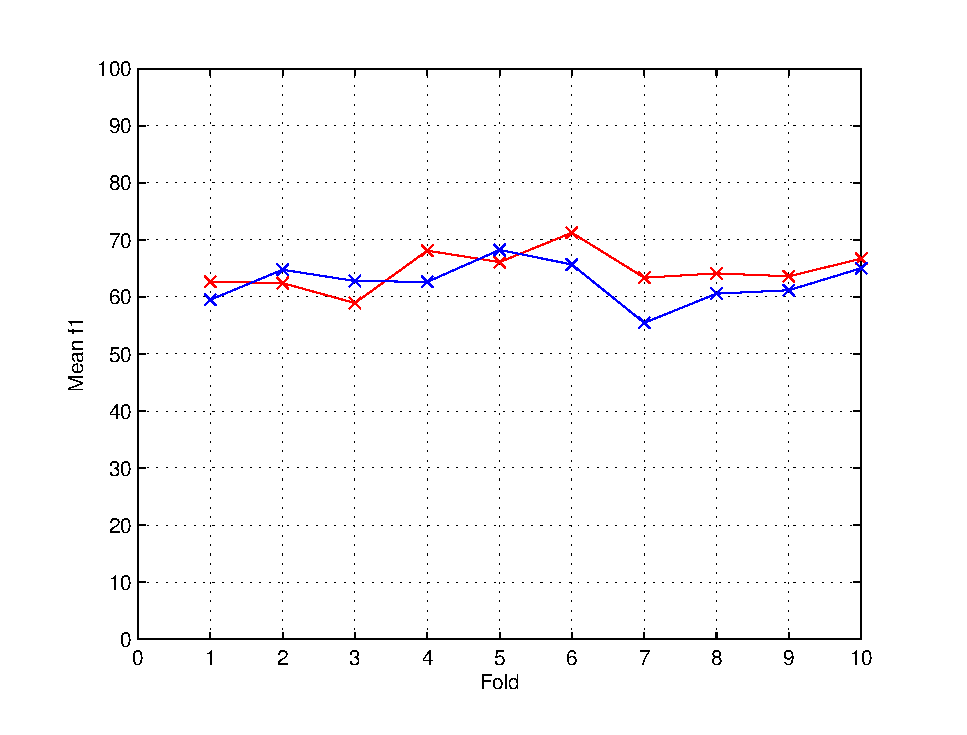
\includegraphics[width=\textwidth]{images/noisy_fold_f1_plot.eps}
     	\caption{Average value of F1 measure for all 6 emotions against folds for noisy data}
     	\label{fig:avgF1Noisy}
    \end{subfigure}
    \caption{Red: Six Output NN, Blue: Single Output NNs}
    \label{fig:avgF1}
\end{figure}

\begin{table}[!ht]
\centering
\begin{tabular}{|l|l|c|c|c|c|c|c|}
	\cline{3-8}
	\multicolumn{2}{c}{}& \multicolumn{6}{ |c| }{Predicted class}\\
	\cline{3-8}
	\multicolumn{2}{c|}{} & 1 Anger & 2 Disgust & 3 Fear & 4 Happiness & 5 Sadness & 6 Surprise\\ \cline{1-8}
	\multirow{6}{*}{Actual class}& 1 Anger & 9.1 & 1.5 & 0.5 & 0.3 & 1.6 & 0.1 \\ \cline{2-8}
	& 2 Disgust & 1.1 & 16.1 & 0.4 & 0.4 & 1.6 & 0.2\\ \cline{2-8}
	& 3 Fear & 0.4 & 0.3 & 9.5 & 0.1 & 0.4 & 1.1 \\ \cline{2-8}
	& 4 Happiness & 0.1 & 0.6 & 0.3 & 20.1 & 0.2 & 0.2 \\ \cline{2-8}
	& 5 Sadness & 1.2 & 2.3 & 0.5 & 0.5 & 8.4 & 0.3 \\ \cline{2-8}
	& 6 Surprise & 0.1 & 0.2 & 0.7 & 0.6 & 0.4 & 18.6\\ \hline
\end{tabular}
\caption{Confusion Matrix of Six Output NN - Clean Data}
\label{tab:sixOutputCleanConfusion}
\end{table}

\begin{table}[!ht]
\centering
\begin{tabular}{|l|l|c|c|c|c|c|c|}
	\cline{3-8}
	\multicolumn{2}{c}{}& \multicolumn{6}{ |c| }{Predicted class}\\
	\cline{3-8}
	\multicolumn{2}{c|}{} & 1 Anger & 2 Disgust & 3 Fear & 4 Happiness & 5 Sadness & 6 Surprise\\ \cline{1-8}
	\multirow{6}{*}{Actual class}& 1 Anger & 1.1 & 1.5 & 2.4 & 0.9 & 2.1 & 0.8 \\ \cline{2-8}
	& 2 Disgust & 0.2 & 15.2 & 1.6 & 0.4 & 0.8 & 0.5\\ \cline{2-8}
	& 3 Fear & 0.3 & 1.4 & 13.7 & 1.1 & 0.5 & 1.7 \\ \cline{2-8}
	& 4 Happiness & 0.2 & 0.6 & 0.6 & 18.4 & 0.4 & 0.6 \\ \cline{2-8}
	& 5 Sadness & 0.6 & 0.8 & 1.4 & 0.3 & 6.8 & 1.1 \\ \cline{2-8}
	& 6 Surprise & 0.1 & 0.3 & 1.4 & 1.1 & 0.8 & 18.3\\ \hline
\end{tabular}
\caption{Confusion Matrix of Six Output NN - Noisy Data}
\label{tab:sixOutputNoisyConfusion}
\end{table}

\begin{table}[!ht]
\centering
\begin{tabular}{|l|l|c|c|c|c|c|c|}
	\cline{3-8}
	\multicolumn{2}{c}{}& \multicolumn{6}{ |c| }{Predicted class}\\
	\cline{3-8}
	\multicolumn{2}{c|}{} & 1 Anger & 2 Disgust & 3 Fear & 4 Happiness & 5 Sadness & 6 Surprise\\ \cline{1-8}
	\multirow{6}{*}{Actual class}& 1 Anger & 9.4 & 1.3 & 0.6 & 0.6 & 1.1 & 0.1 \\ \cline{2-8}
	& 2 Disgust & 1.2 & 15.9 & 0.3 & 0.7 & 1.6 & 0.1\\ \cline{2-8}
	& 3 Fear & 0.7 & 0.2 & 9.6 & 0 & 0.4 & 0.9 \\ \cline{2-8}
	& 4 Happiness & 0.1 & 0.7 & 0 & 20.2 & 0.3 & 0.2 \\ \cline{2-8}
	& 5 Sadness & 0.8 & 1.7 & 0.5 & 0.4 & 9.6 & 0.2 \\ \cline{2-8}
	& 6 Surprise & 0 & 0.4 & 0.9 & 0.4 & 0.3 & 18.6\\ \hline
\end{tabular}
\caption{Confusion Matrix of Six Single Output NNs - Clean Data}
\label{tab:sixSingleOutputsCleanConfusion}
\end{table}

\begin{table}[!ht]
\centering
\begin{tabular}{|l|l|c|c|c|c|c|c|}
	\cline{3-8}
	\multicolumn{2}{c}{}& \multicolumn{6}{ |c| }{Predicted class}\\
	\cline{3-8}
	\multicolumn{2}{c|}{} & 1 Anger & 2 Disgust & 3 Fear & 4 Happiness & 5 Sadness & 6 Surprise\\ \cline{1-8}
	\multirow{6}{*}{Actual class}& 1 Anger & 1.6 & 1.7 & 2 & 1.1 & 2.1 & 0.3 \\ \cline{2-8}
	& 2 Disgust & 0.2 & 15.6 & 1.4 & 0.7 & 0.6 & 0.2\\ \cline{2-8}
	& 3 Fear & 0.5 & 2 & 12 & 1 & 1 & 2.2 \\ \cline{2-8}
	& 4 Happiness & 0.1 & 0.7 & 1 & 17.9 & 0.5 & 0.6 \\ \cline{2-8}
	& 5 Sadness & 1.3 & 1 & 1.4 & 0.5 & 5.6 & 1.2 \\ \cline{2-8}
	& 6 Surprise & 0.2 & 0.6 & 1.5 & 0.5 & 1 & 18.2\\ \hline
\end{tabular}
\caption{Confusion Matrix of Six Single Output NNs - Noisy Data}
\label{tab:sixSingleOutputsNoisyConfusion}
\end{table}

\begin{table}[!ht]
\centering
\begin{tabular}{|l|c|c|c|}
	\cline{3-3}
	\multicolumn{2}{c|}{} & Average Classification Rate \\ \cline{1-3}
	\multirow{2}{*}{Network}& Six Output (Clean) & 0.8180  \\ \cline{2-3}  
	& Six Output (Noisy) & 0.7350  \\ \cline{2-3} 
		& Single Outputs (Clean) & 0.8330 \\ \cline{2-3} 
	& Single Outputs (Noisy) & 0.7090 \\ \hline

\end{tabular}
\caption{Average Classification Rate}
\label{tab:avgClassificationRate}
\end{table}

\begin{table}[!ht]
\centering
\begin{tabular}{|l|c|c|c|c|c|c|c|}
	\cline{3-8}
	\multicolumn{2}{c}{}& \multicolumn{6}{ |c| }{Class}\\
	\cline{3-8}
	\multicolumn{2}{c|}{} & 1 Anger & 2 Disgust & 3 Fear & 4 Happiness & 5 Sadness & 6 Surprise\\ \cline{1-8}
	\multirow{2}{*}{Network}& Six Output (Clean) & 69.4656 & 81.3131 & 80.5085 & 93.4884 & 63.6364 & 90.2913 \\ \cline{2-8}  
	& Six Output (Noisy) & 12.5 & 81.2834 & 73.2620 & 88.4615 & 61.8182 & 83.1818 \\ \cline{2-8} 
		& Single Outputs (Clean) & 71.7557 & 80.3030 & 81.3559 & 93.9535 & 72.7273 & 90.2913\\ \cline{2-8} 
	& Single Outputs (Noisy) & 18.1818 & 83.4225 & 64.1711 & 86.0577 & 50.9091 & 82.7273\\ \hline

\end{tabular}
\caption{Recall Per Class}
\label{tab:recallPerClass}
\end{table}

\begin{table}[!ht]
\centering
\begin{tabular}{|l|c|c|c|c|c|c|c|}
	\cline{3-8}
	\multicolumn{2}{c}{}& \multicolumn{6}{ |c| }{Class}\\
	\cline{3-8}
	\multicolumn{2}{c|}{} & 1 Anger & 2 Disgust & 3 Fear & 4 Happiness & 5 Sadness & 6 Surprise\\ \cline{1-8}
	\multirow{2}{*}{Network}& Six Output (Clean) & 75.8333 & 76.6667 & 79.8319 & 91.3636 & 66.6667 & 90.07317 \\ \cline{2-8}  
	& Six Output (Noisy) & 44 & 76.7677 & 64.9289 & 82.8829 & 59.6491 & 79.5652 \\ \cline{2-8} 
		& Single Outputs (Clean) & 77.0492 & 78.7129 & 80.6723 & 90.5830 & 72.1805 & 92.5373\\ \cline{2-8} 
	& Single Outputs (Noisy) & 41.0256 & 72.2222 & 62.1762 & 82.4885 & 51.8519 & 80.1762\\ \hline

\end{tabular}
\caption{Precision Per Class}
\label{tab:precisionPerClass}
\end{table}

\begin{table}[!ht]
\centering
\begin{tabular}{|l|c|c|c|c|c|c|c|}
	\cline{3-8}
	\multicolumn{2}{c}{}& \multicolumn{6}{ |c| }{Class}\\
	\cline{3-8}
	\multicolumn{2}{c|}{} & 1 Anger & 2 Disgust & 3 Fear & 4 Happiness & 5 Sadness & 6 Surprise\\ \cline{1-8}
	\multirow{2}{*}{Network}& Six Output (Clean) & 72.51 & 78.9216 & 80.1688 & 92.4138 & 65.1163 & 90.5109 \\ \cline{2-8}  
	& Six Output (Noisy) & 19.4690 & 78.9610 & 68.8442 & 85.5814 & 60.7143 & 81.3333 \\ \cline{2-8} 
		& Single Outputs (Clean) & 74.3083 & 79.5 & 81.0127 & 92.2374 & 72.4528 & 91.4005\\ \cline{2-8} 
	& Single Outputs (Noisy) & 25.1969 & 77.4194 & 63.1579 & 84.2353 & 51.3761 & 81.4318\\ \hline

\end{tabular}
\caption{F1 Measure Per Class}
\label{tab:f1MeasurenPerClass}
\end{table}

\begin{figure}[!ht]
	\centering
	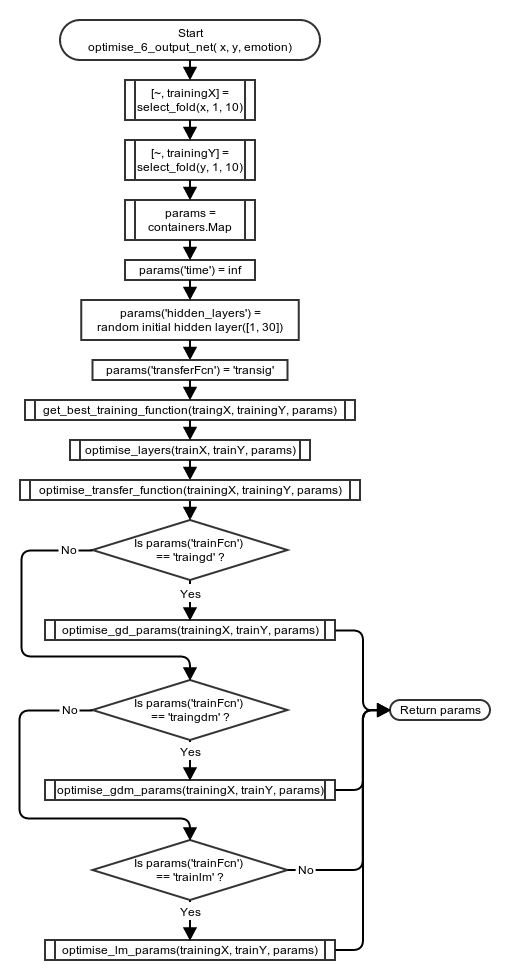
\includegraphics[scale=0.7]{images/flow_chart/optimise_6_output_net.png}
	\caption{Flowchart of \tt{optimise\_6\_output\_net}}
	\label{fig:optimise_6_output_net}
\end{figure}

\begin{figure}[!ht]
	\centering
	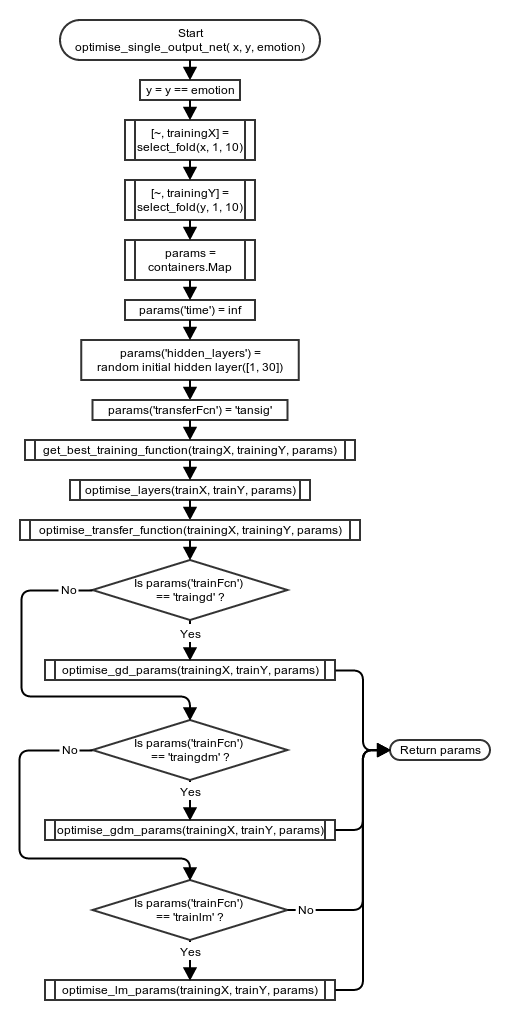
\includegraphics[scale=0.7]{images/flow_chart/optimise_single_output_net.png}
	\caption{Flowchart of \tt{optimise\_single\_output\_net}}
	\label{fig:optimise_single_output_net}
\end{figure}

\begin{figure}[!ht]
	\centering
	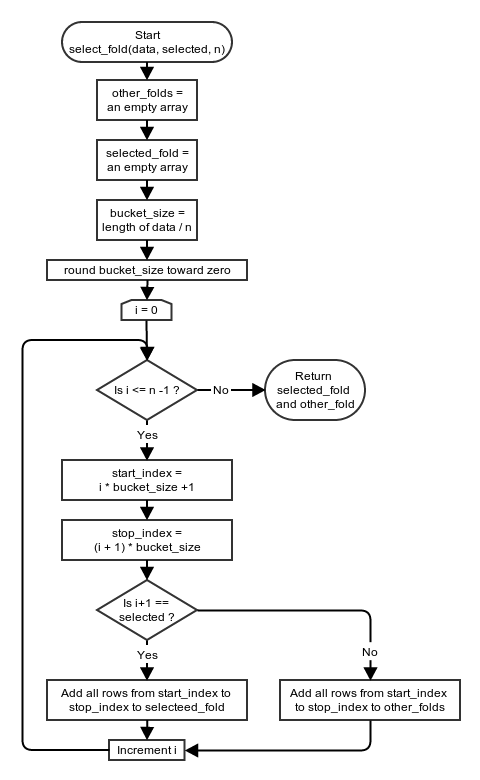
\includegraphics[scale=0.8]{images/flow_chart/select_fold.png}
	\caption{Flowchart of \tt{select\_fold}}
	\label{fig:select_fold}
\end{figure}

\begin{figure}[!ht]
	\centering
	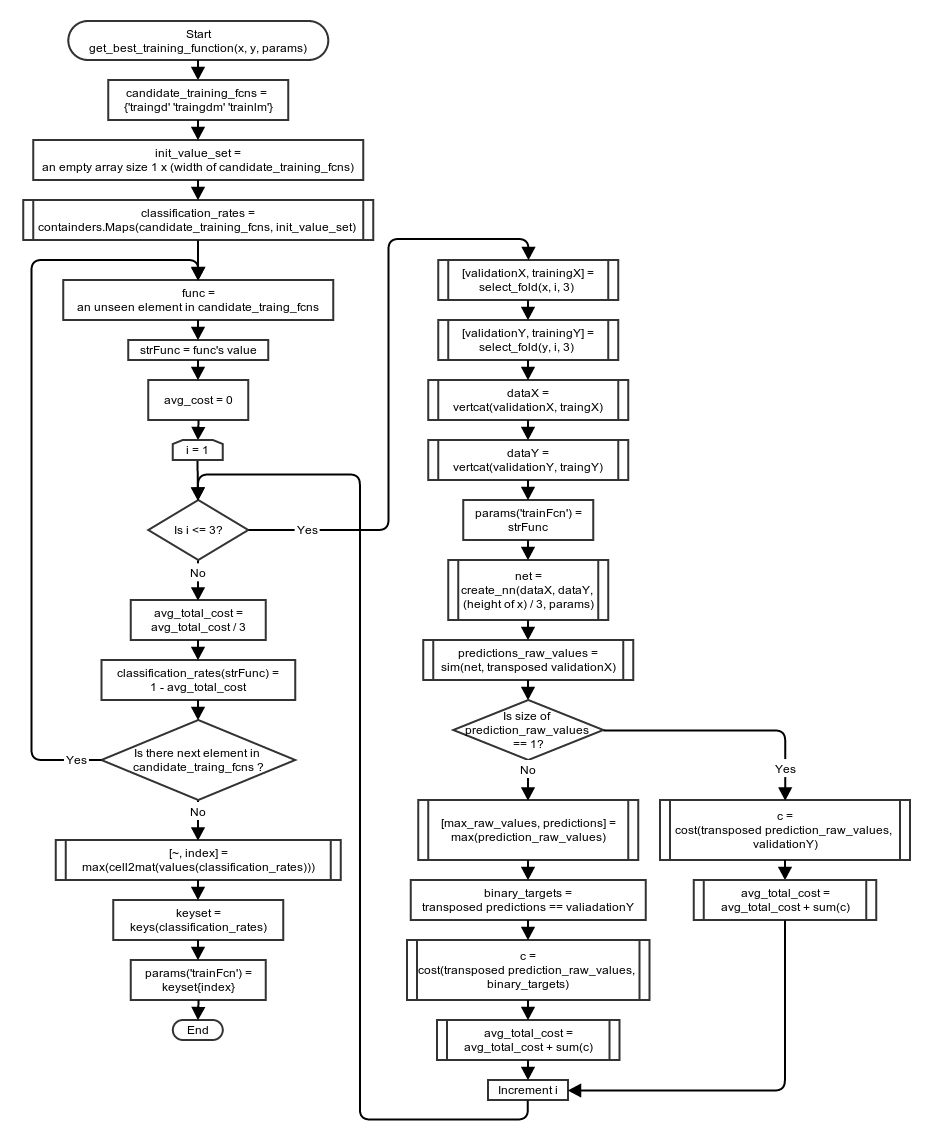
\includegraphics[height=\textheight, width=\textwidth]{images/flow_chart/get_best_training_function.png}
	\caption{Flowchart of \tt{get\_best\_training\_function}}
	\label{fig:get_best_training_function}
\end{figure}

\begin{figure}[!ht]
	\centering
	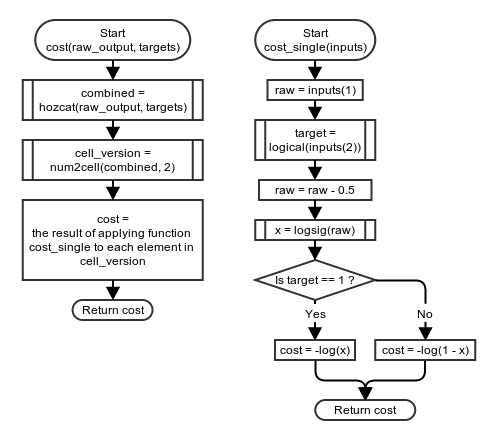
\includegraphics[scale=0.7]{images/flow_chart/cost.png}
	\caption{Flowchart of \tt{cost}}
	\label{fig:cost}
\end{figure}

\begin{figure}[!ht]
	\centering
	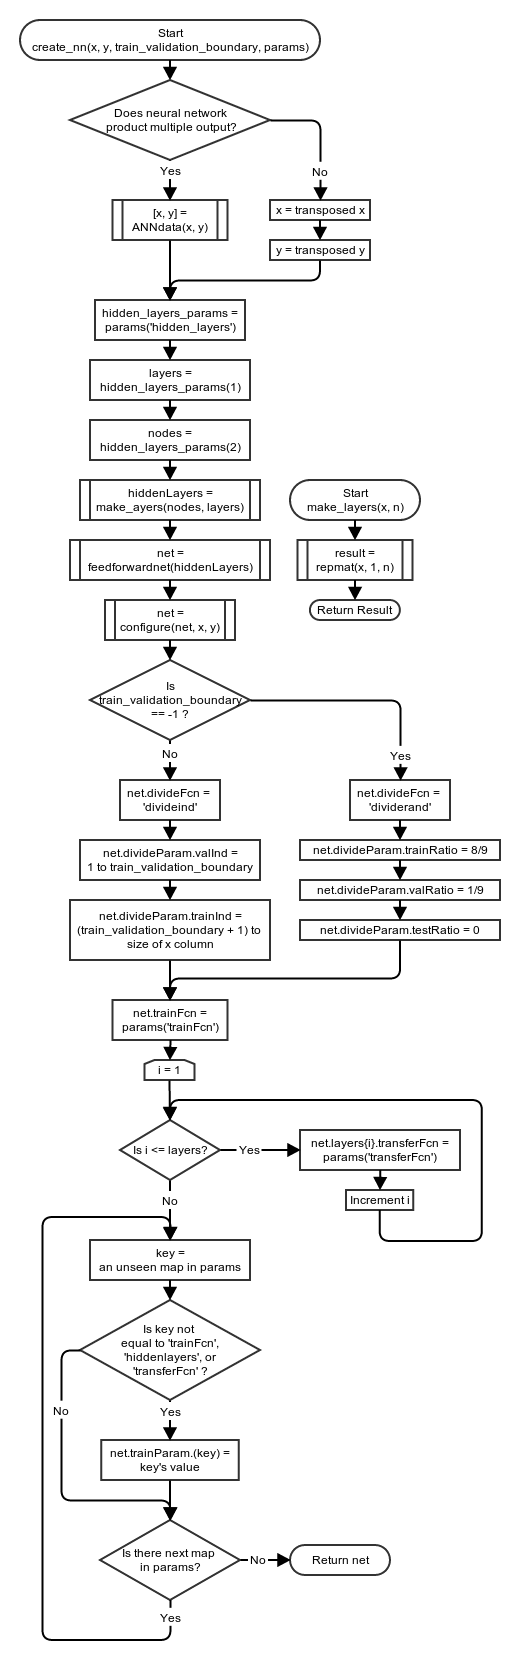
\includegraphics[scale=0.45]{images/flow_chart/create_nn.png}
	\caption{Flowchart of \tt{create\_nn}}
	\label{fig:create_nn}
\end{figure}

\begin{figure}[!ht]
	\centering
	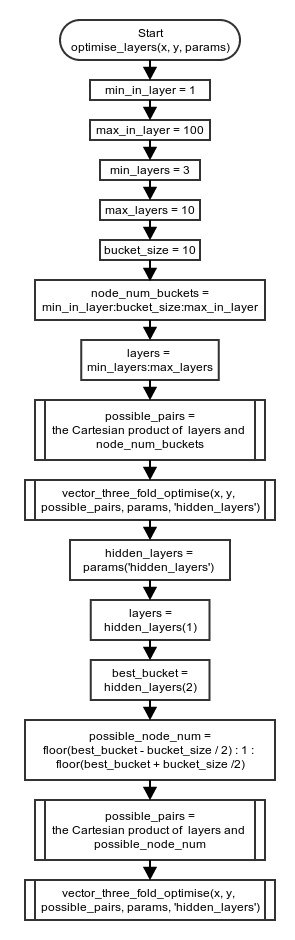
\includegraphics[scale=0.7]{images/flow_chart/optimise_layer.png}
	\caption{Flowchart of \tt{optimise\_layer}}
	\label{fig:optimise_layer}
\end{figure}

\begin{figure}[!ht]
	\centering
	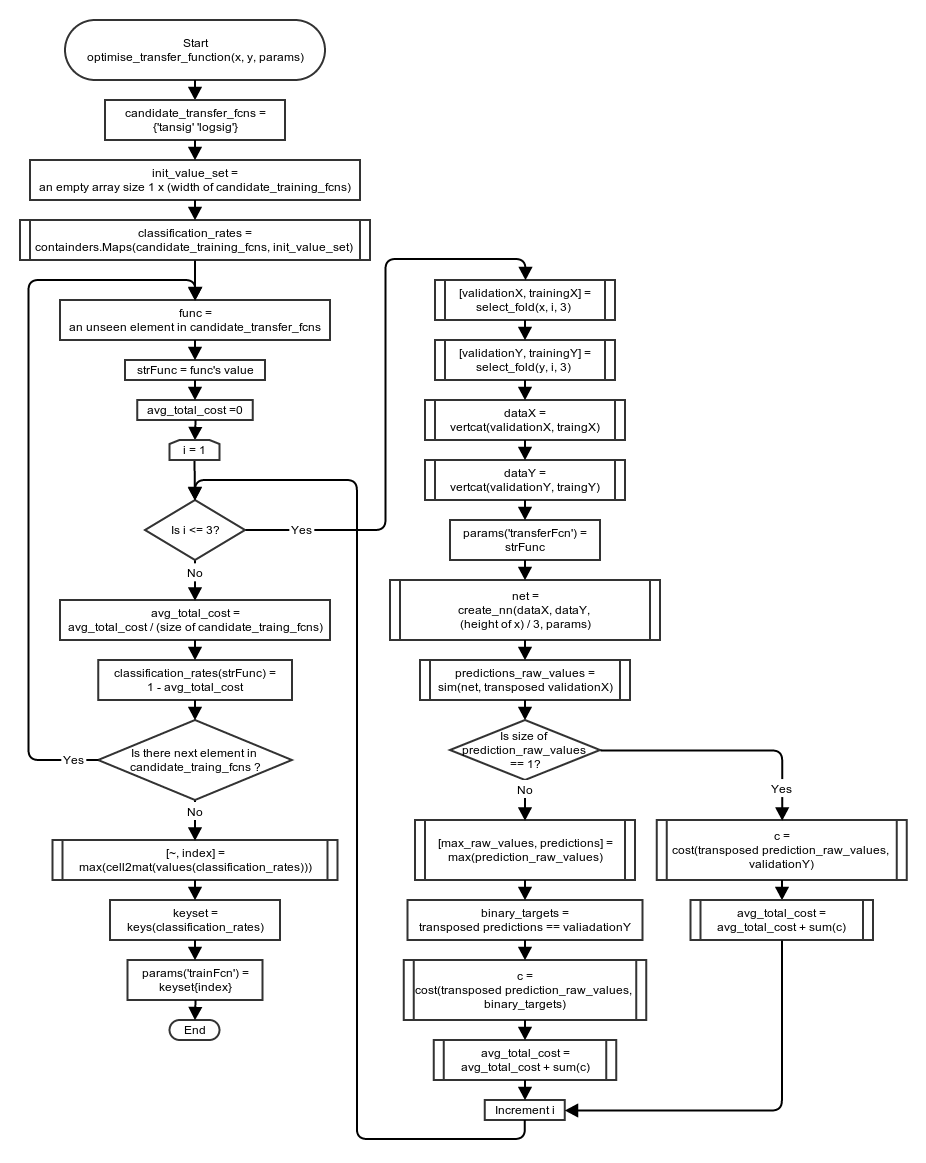
\includegraphics[height=\textheight, width=\textwidth]{images/flow_chart/optimise_transfer_function.png}
	\caption{Flowchart of \tt{optimise\_transfer\_function}}
	\label{fig:optimise_transfer_function}
\end{figure}

\begin{figure}[!ht]
	\centering
	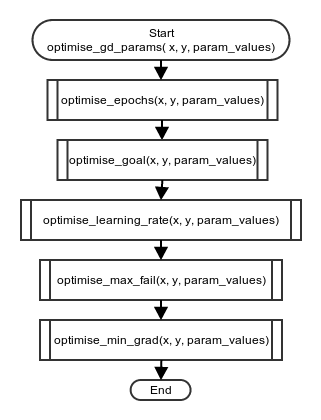
\includegraphics[scale=0.7]{images/flow_chart/optimise_gd_params.png}
	\caption{Flowchart of \tt{optimise\_gd\_params}}
	\label{fig:optimise_gd_params}
\end{figure}

\begin{figure}[!ht]
	\centering
	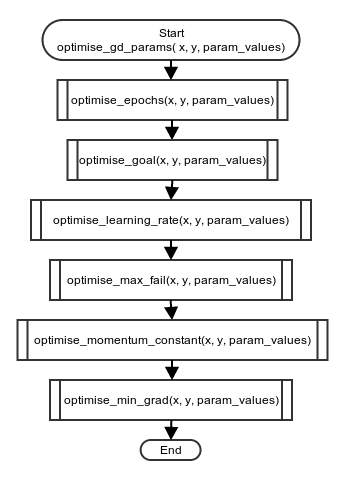
\includegraphics[scale=0.7]{images/flow_chart/optimise_gdm_params.png}
	\caption{Flowchart of \tt{optimise\_gdm\_params}}
	\label{fig:optimise_gdm_params}
\end{figure}

\begin{figure}[!ht]
	\centering
	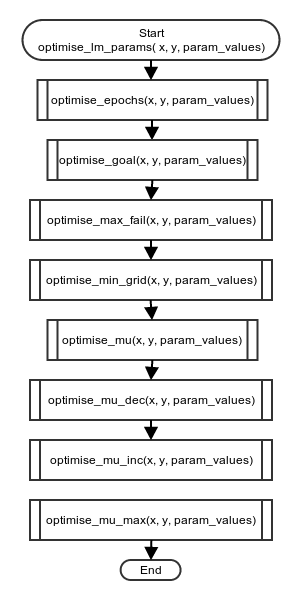
\includegraphics[scale=0.7]{images/flow_chart/optimise_lm_params.png}
	\caption{Flowchart of \tt{optimise\_lm\_params}}
	\label{fig:optimise_lm_params}
\end{figure}

\begin{figure}[!ht]
	\centering
	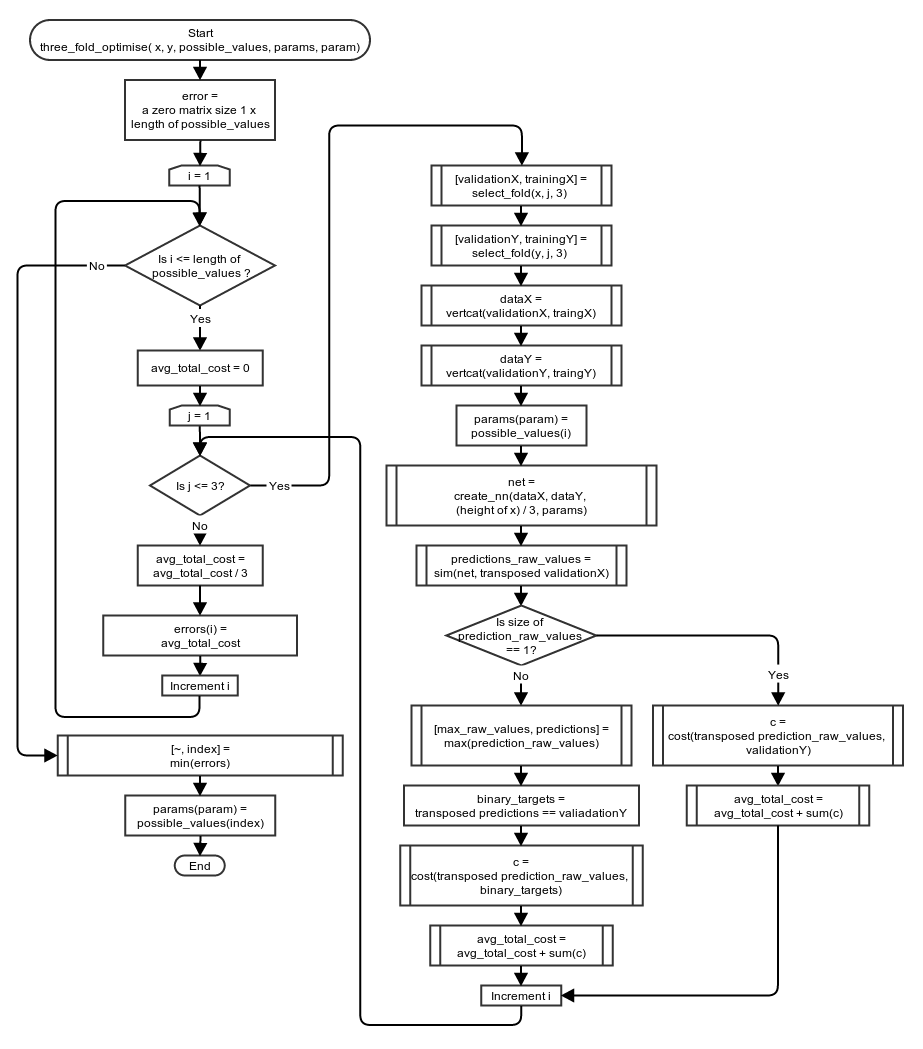
\includegraphics[height=\textheight, width=\textwidth]{images/flow_chart/three_fold_optimise.png}
	\caption{Flowchart of \tt{three\_fold\_optimise}}
	\label{fig:three_fold_optimise}
\end{figure}

\begin{figure}[!ht]
	\centering
	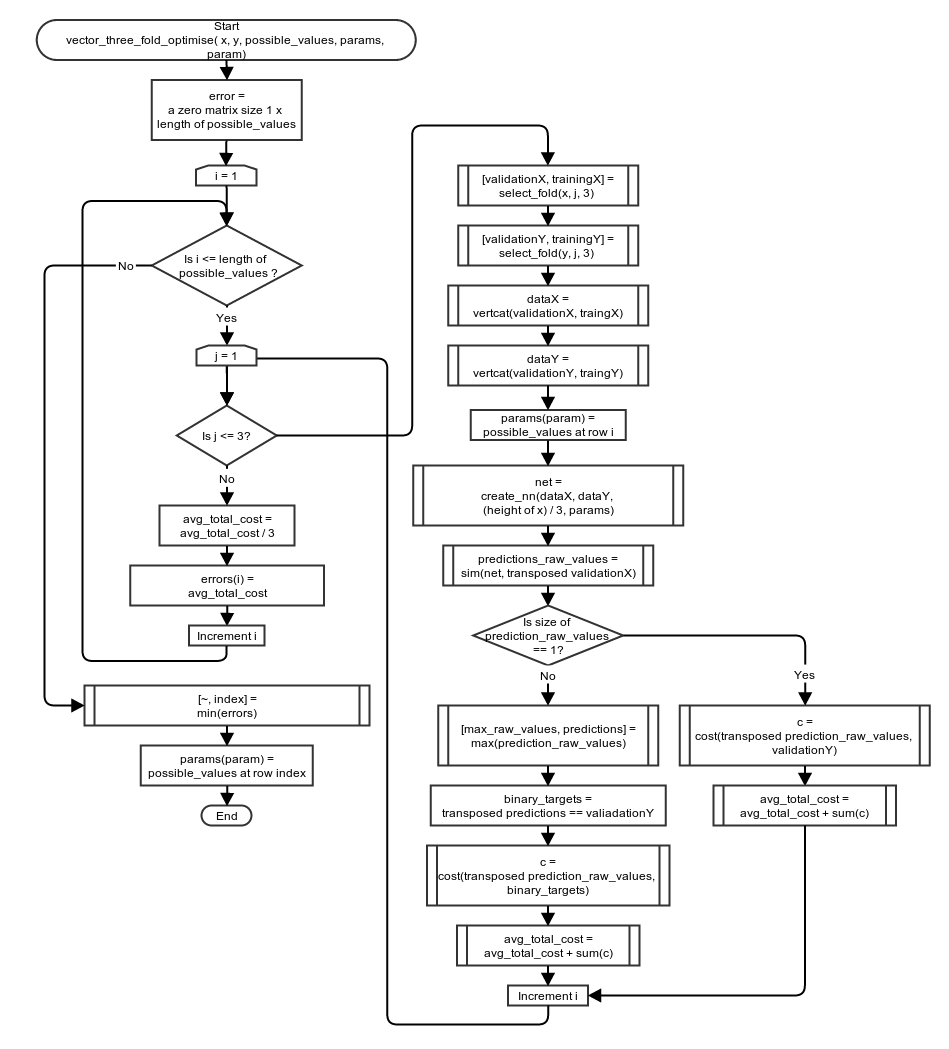
\includegraphics[height=\textheight, width=\textwidth]{images/flow_chart/vector_three_fold_optimise.png}
	\caption{Flowchart of \tt{vector\_three\_fold\_optimise}}
	\label{fig:vector_three_fold_optimise}
\end{figure}

\begin{figure}[!ht]
	\centering
	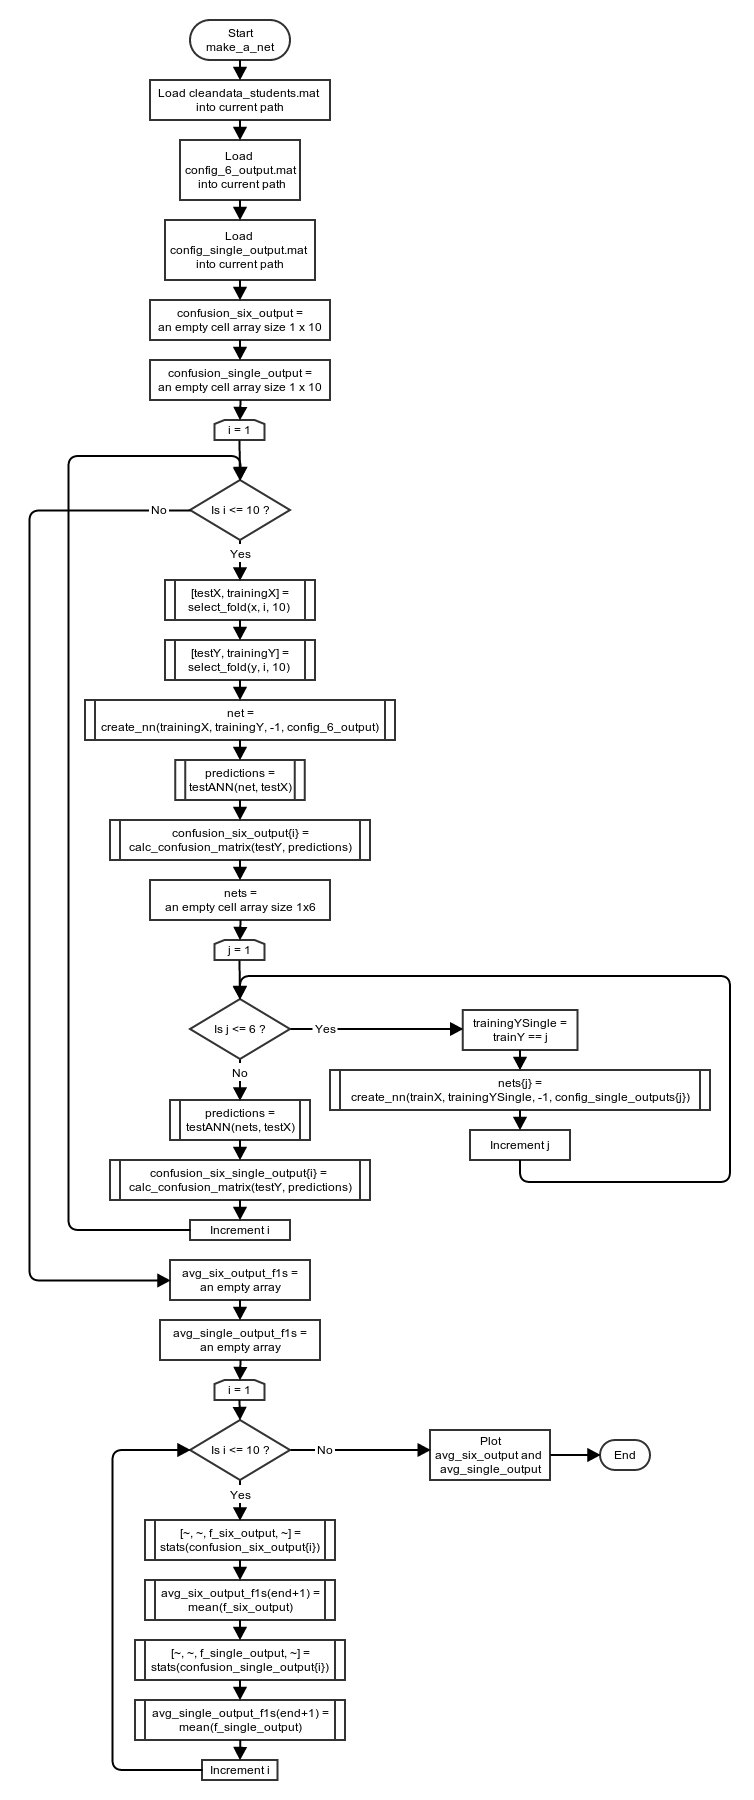
\includegraphics[height=\textheight, width=\textwidth]{images/flow_chart/make_a_net.png}
	\caption{Flowchart of \tt{make\_a\_net}}
	\label{fig:make_a_net}
\end{figure}

\begin{figure}[!ht]
	\centering
	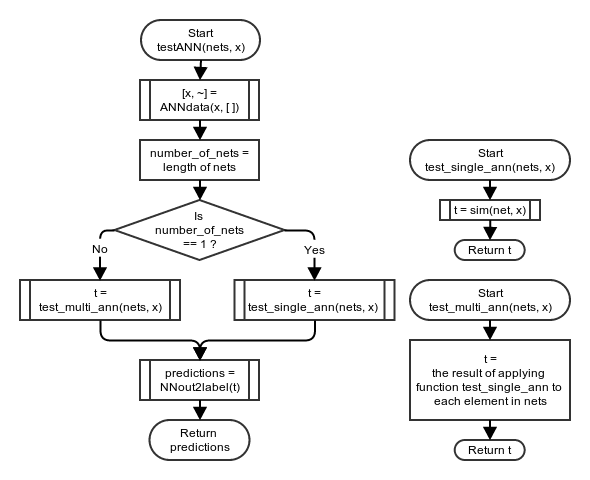
\includegraphics[scale=0.63]{images/flow_chart/testann.png}
	\caption{Flowchart of \tt{testANN}}
	\label{fig:testann}
\end{figure}

\begin{figure}[!ht]
	\centering
	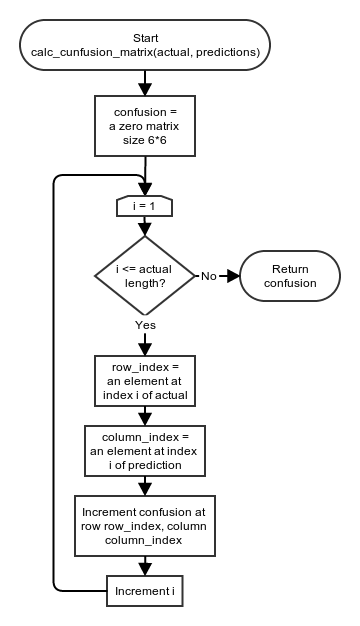
\includegraphics[scale=0.63]{images/flow_chart/cal_cunfusion_matrix.png}
	\caption{Flowchart of \tt{cal\_cunfusion\_matrix}}
	\label{fig:cal_cunfusion_matrix}
\end{figure}

\end{document}
